\documentclass{article}


\usepackage{chinese}
\usepackage{listings}

\lstset{frame=tb,
  language=Python,
}

\title{深度學習模型的比較研究 -- 以 MNIST 為例}

\author{
  陳鍾誠\thanks{Use footnote for providing further
    information about author (webpage, alternative
    address)---\emph{not} for acknowledging funding agencies.} \\
  國立金門大學 資訊工程學系\\
  \texttt{ccc@nqu.edu.tw} \\
}

\begin{document}
\maketitle

\begin{abstract}
本論文的開放原始碼專案網址為:\url{ https://github.com/cccresearch/nnModelCompare }
\\
\\
不同的神經網路模型,經訓練之後的正確率可能差異很大。本文針對手寫數字辨識的MNIST 資料庫進行測試,以便觀察模型的表現,並分析其背後的原因。
\end{abstract}


% keywords can be removed
\keywords{神經網路\and 深度學習\and MNIST}


\section{簡介}

近幾年 深度學習技術 讓人工智慧領域有了很大的進展,也吸引到了學術界與產業界共同投入研究,相繼開發出更好,但也相對更複雜的模型。

為何有些模型表現好,有些模型表現差,各個網路層的效用是甚麼,為何需要加入某些層,若拿掉的話會有甚麼不良反應嗎?這就是本研究所想要探討的問題!

\section{背景}
\label{background}

手寫數字辨識的 MNIST 是影像辨識領域中最常被拿來測試的資料集,而 CNN 卷積神經網路架構的 LeNet 則是 Yann Le Cun 1989 年在研究手寫辨識問題時,提出來的辨識模型,實驗發現 LeNet 在手寫辨識上有相當高的正確率。

不過,其他的模型,像是使用多層感知器,也可以達到 90\% 以上的正確率,


 \cite{kour2014real,kour2014fast} and see \cite{hadash2018estimate}.

The documentation for \verb+natbib+ may be found at
\begin{center}
  \url{http://mirrors.ctan.org/macros/latex/contrib/natbib/natnotes.pdf}
\end{center}
Of note is the command \verb+\citet+, which produces citations
appropriate for use in inline text.  For example,
\begin{verbatim}
   \citet{hasselmo} investigated\dots
\end{verbatim}
produces
\begin{quote}
  Hasselmo, et al.\ (1995) investigated\dots
\end{quote}

\begin{center}
  \url{https://www.ctan.org/pkg/booktabs}
\end{center}


\section{方法}

簡易的『爬山演算法』如下圖所示
1 所示。

\begin{verbatim}
Algorithm Hill-Climbing(pi)
 p = pi // 設定粒子 p 為起始粒子 pi
 while not isEnd()
 pn = p.neighbor(step) //選擇粒子 p 的鄰居 pn
 if pn.fitness()>=p.fitness() //如果更好,就接受
 p = pn;
End Algorithm
\end{verbatim}

\begin{lstlisting}
def hillClimbing(s, maxGens, maxFails):   # 爬山演算法的主體函數
    print("start: ", s.str())             # 印出初始解
    fails = 0                             # 失敗次數設為 0
    # 當代數 gen<maxGen,且連續失敗次數 fails < maxFails 時,就持續嘗試尋找更好的解。
    for gens in range(maxGens):
        snew = s.neighbor()               #  取得鄰近的解
        sheight = s.height()              #  sheight=目前解的高度
        nheight = snew.height()           #  nheight=鄰近解的高度
        if (nheight >= sheight):          #  如果鄰近解比目前解更好
            print(gens, ':', snew.str())  #    印出新的解
            s = snew                      #    就移動過去
            fails = 0                     #    移動成功,將連續失敗次數歸零
        else:                             #  否則
            fails = fails + 1             #    將連續失敗次數加一
        if (fails >= maxFails):
            break
    print("solution: ", s.str())          #  印出最後找到的那個解
    return s                              #    然後傳回。
\end{lstlisting}

\begin{center}
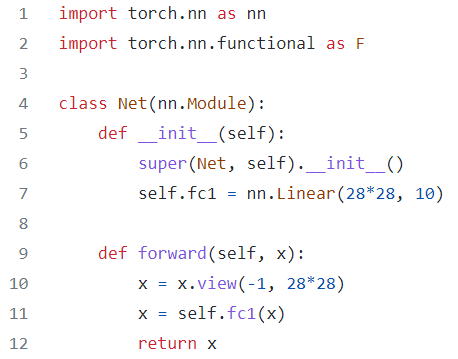
\includegraphics{./img/fc1.png}
\end{center}

\subsection{高度函數如何設計}

Measure Measure Measure Measure Measure Measure Measure Measure Measure Measure Measure Measure Measure Measure 

\begin{equation}
\xi _{ij}(t)=P(x_{t}=i,x_{t+1}=j|y,v,w;\theta)= {\frac {\alpha _{i}(t)a^{w_t}_{ij}\beta _{j}(t+1)b^{v_{t+1}}_{j}(y_{t+1})}{\sum _{i=1}^{N} \sum _{j=1}^{N} \alpha _{i}(t)a^{w_t}_{ij}\beta _{j}(t+1)b^{v_{t+1}}_{j}(y_{t+1})}}
\end{equation}

\subsubsection{如何選取好的鄰居?}

任何的參數變動,都可以創造出新的鄰居模型,因此、鄰居的選擇性是無限多的,我們面臨的問題是,該如何從無限多的鄰居當中,選擇一個有可能更好的適當鄰居呢?

在此、我們用了一些啟發式法則如下

\begin{enumerate}  
\item 加一個新層 
\item 將一層換成另一層
\item 調整某層的參數
\end{enumerate}

\paragraph{Paragraph}

Paragraph Paragraph Paragraph Paragraph Paragraph Paragraph Paragraph Paragraph Paragraph Paragraph Paragraph Paragraph Paragraph Paragraph 

\section{實驗}
\label{sec:others}

\begin{table}
 \caption{不同模型的 MNIST 正確率}
  \centering
  \begin{tabular}{lll}
    模型     & 正確率     & 說明 \\
    \midrule
    fc1 & 74\% &       \\
    fc1s & 92\% &       \\
    fc2 & 10\% & 損失負無限大 \\
    fc2s & 92\% &       \\
    fc2net & 95\% &       \\
    fc2signet & 91\% &       \\
    LeNet & 97\%  &      \\
    \bottomrule
  \end{tabular}
  \label{tab:table}
\end{table}

 \cite{kour2014real,kour2014fast} and see \cite{hadash2018estimate}.

The documentation for \verb+natbib+ may be found at
\begin{center}
  \url{http://mirrors.ctan.org/macros/latex/contrib/natbib/natnotes.pdf}
\end{center}
Of note is the command \verb+\citet+, which produces citations
appropriate for use in inline text.  For example,
\begin{verbatim}
   \citet{hasselmo} investigated\dots
\end{verbatim}
produces
\begin{quote}
  Hasselmo, et al.\ (1995) investigated\dots
\end{quote}

\begin{center}
  \url{https://www.ctan.org/pkg/booktabs}
\end{center}


\subsection{Figures}
\lipsum[10] 
See Figure \ref{fig:fig1}. Here is how you add footnotes. \footnote{Sample of the first footnote.}
\lipsum[11] 

\begin{figure}
  \centering
  \fbox{\rule[-.5cm]{4cm}{4cm} \rule[-.5cm]{4cm}{0cm}}
  \caption{Sample figure caption.}
  \label{fig:fig1}
\end{figure}

\subsection{Tables}
\lipsum[12]
See awesome Table~\ref{tab:table}.

\begin{table}
 \caption{Sample table title}
  \centering
  \begin{tabular}{lll}
    \toprule
    \multicolumn{2}{c}{Part}                   \\
    \cmidrule(r){1-2}
    Name     & Description     & Size ($\mu$m) \\
    \midrule
    Dendrite & Input terminal  & $\sim$100     \\
    Axon     & Output terminal & $\sim$10      \\
    Soma     & Cell body       & up to $10^6$  \\
    \bottomrule
  \end{tabular}
  \label{tab:table}
\end{table}

\subsection{Lists}
\begin{itemize}
\item Lorem ipsum dolor sit amet
\item consectetur adipiscing elit. 
\item Aliquam dignissim blandit est, in dictum tortor gravida eget. In ac rutrum magna.
\end{itemize}

\renewcommand\refname{參考文獻}

\bibliographystyle{unsrt}  
\bibliography{references}  %%% Remove comment to use the external .bib file (using bibtex).
%%% and comment out the ``thebibliography'' section.


%%% Comment out this section when you \bibliography{references} is enabled.
%\begin{thebibliography}{1}

% \end{thebibliography}


\end{document}
